\documentclass[prl,twocolumn]{revtex4-1}
\usepackage{graphicx}
\usepackage{amsmath}
\usepackage{hyperref}
\usepackage{booktabs}
\usepackage{xcolor}

\usepackage{siunitx}

\setlength{\tabcolsep}{10pt}

\newenvironment{sistema}%
  {\left\lbrace\begin{array}{@{}l@{}}}%
  {\end{array}\right.}



\begin{document}
\title{Gelation as a condensation frustrated by hydrodynamics and mechanical tension}
\author{Hideyo Tsurusawa}
\thanks{These authors contributed equally to this work}
\author{Mathieu Leocmach}
\thanks{These authors contributed equally to this work}
\author{Hajime Tanaka}
\email{tanaka@iis.u-tokyo.ac.jp}
\affiliation{ {Institute of Industrial Science, University of Tokyo, 4-6-1 Komaba, Meguro-ku, Tokyo 153-8505, Japan} }

\begin{abstract}

\end{abstract}

\maketitle

\section*{Introduction} 



\section*{Results}

\subsection*{Observation of the initial stage}

We use a novel experimental set-up that allows the observation of the entire process of gelation at a single particle level (see Methods). In a suspension of sticky colloids with long range repulsion, we suddenly turn off the repulsion. The short range attraction become dominant, eventually leading to the formation of a gel. The whole process takes place on the microscope stage and can thus be observed dynamically in three dimensions from the very beginning.

Our protocol is not equivalent to a redispersion of an existing gel at the same state point either by shaking or shear melting like in  e.g.~\cite{lu2008gelation,Teece2011,Bartlett2012}. It is closer to a quench, however we expect differences compared to a quench simulated via molecular or Brownian dynamics, because of the presence of a solvent mediating hydrodynamic interactions~\cite{Furukawa2010}. Thus our protocol might be very close to application relevant processes where the sudden addition of a component (e.g. salt, acid, depletion agent) induces aggregation in an otherwise stable suspension (e.g. milk).

Figure~\ref{fig:methods}c-h shows a computer reconstruction from experimental coordinates of a typical gelation experiment. We are able to follow the state of the system from (Fig.~\ref{fig:methods}c) a Wigner crystal where the particles are far apart due to repulsion to (Fig.~\ref{fig:methods}h) a fully percolated network. Using this protocol, we explored the phase diagram (Fig.~\ref{fig:methods}b) and found three possible behaviours: permanent gelation as above, transient gelation and cluster formation. Transient gelation is characterised by the formation of a percolating network that melts into separate clusters over a few tens of Brownian times (the time needed for an isolated particle to diffuse over its own radius, here about $\SI{10}{second}$).

We observe in Fig.~\ref{fig:methods}b that the spinodal line predicted by the generalized free volume theory~\cite{Fleer2008} corresponds roughly to the boundary between permanent and transient gelation. Furthermore, it means that in our system gelation can happen transiently without an underlying spinodal decomposition dynamics, somewhat in contradiction to~\cite{lu2008gelation}.





\section{Cluster aggregation} % Subject I: Cluster formation
% Topic sentence
Figure~\ref{fig:methods}a shows the phase diagram of all samples.
First of all, we focus on cluster formation since clusters constitute ``building blocks'' of gels.
% Results of birth
Figure~\ref{fig:fluid_dilute} a shows the compaction dynamics of the clusters with three colloids in the early stage.
The results show that the clusters can hardly accomplish compaction within one Brownian motion time and clusters with four and five colloids show very similar tendency (Supplement).
% Explanation 1) Local energy minimization.
If one assumes that each colloid can move independently by Brownian motion and static short-range attractions are induced between colloids, the clusters with three colloids should reach the compact states within one Brownian motion time.
This explanation contradicts to our results.
% Addressing our question
In other words, some interactions stabilize linear structures, competing with the principle of energy minimization.
% Explanation 2) Electrostatic repulsion.
Although the effect of electrostatic repulsions has been studied, our results are observed after salt screens surface charges and electrostatic repulsions can be negligible in our system.
% Explanation 3) Hydrodynamic interactions.
Thus, the only possible explanation is the effect of hydrodynamic interactions.
Hydrodynamic interactions originate from the incompressivility of the solvent, whose effect between colloids have been demonstrated by both numerical simulations and the experiments of optical tweezers.
For compaction, clusters must squeeze the solvent inside the cluster to the outside.
% Conclusion.
Our results suggest that squeezing process can be the bottleneck of compaction and hydrodynamic interactions enhance linear structures in clusters.



% Results of growth
% topic sentence
To investigate whether clusters can reach compact states in their growing stage, fractal dimension of each time is analysed in Figure~\ref{fig:fluid_dilute}b.
% General explanation about fractal dimension.
In general, compact clusters have df around three, whereas chain-like clusters have df around one.
%Our results of fractal dimensions
Our results show that df increases from 1 in the early stage to 2 in the late stage but df is much lower than three.
% Explanation 1) DLCA
Previously diffusion limited cluster aggregation model has been proposed to explain uncompact structures of clusters, assuming sticky attractions.
But DLCA model predicts that df is always fixed around 1.85, which contradicts to our results.
% Addressing our question
Therefore, other mechanism should decrease df close to 1 from condensation equilibrium.
% Explanation 2) Hydrodynamic interactions
As discussed in the early stage of cluster formation, hydrodynamic interactions can frustrate condensation of clusters.
If clusters form chain-like structures, clusters can both avoid squeezing process and decrease resistance from external flow.
Therefore, structures of df = 1 are hydrodynamically favored though energetically disfavored.
% Conclusion
Our results suggest that hydrodynamic interactions dominate the system in the early stage.
As the cluster aggregation proceeds, each colloid can access to a more compact state, squeezing out the solvent in the cluster, and df gradually increases.




\section{Dilute gels} % Subject II: Dilute gels
% Topic sentence
Next, we focus on the mechanism of gelation in a dilute system.
% Our results
Figure~\ref{fig:general}c-h shows the process of gelation of phi = 7\%.
Clusters grow by connecting with each other and the radius of gyration of the biggest cluster finally becomes comparable to the system size as shown in Figure~\ref{fig:fluid_dilute}c. 
Figure~\ref{fig:fluid_dilute}b shows that fractal dimension of clusters increase from 1 in the early stage to 2 in the late stage as similar with the case of cluster aggregation.
% Addressing our question
One can address a natural question about dilute gels: Why can the system percolate with phi of only 7\%?
% Introduction to effective phi
Number density of colloids has little importance since fractal dimension of the system is much lower than three and it changes during the gelation process.
% Procedure to calculate the effective volume
To calculate the ‘ effective ’ volume fraction of colloid, we replace each cluster with the effective sphere whose radius is equal to the radius gyration of the cluster.
% Results of effective phi
As shown in Figure~\ref{fig:fluid_dilute}, the effective volume fraction increases from 7\% in the early stage to 60\% in the late stage.
% Discuss the mechanism of percolation in a dilute gel
Our results clearly reveal that the system cannot avoid percolation because the effective volume fraction is too high.
The reason for the 10 times increase of the effective phi is that df is much lower than three.
The low df originates from hydrodynamic interactions.
% Conclusion
Therefore, percolation in a dilute system is a consequence of condensation frustrated by hydrodynamic interactions.





\section{Dense gels} % Subject III: Dense gels
% Topic sentence
Gelation in a dense system, on the other hand, behaves different patterns than in a dilute system.
% Results of the entire process of dense gelation
As shown in Figure~\ref{fig:dense}a, the system accomplishes percolation in a few minutes, whereas coarsening process proceeds for several hours.
% Focusing on percolation mechanism
% Results of percolation
When the system percolates at t = 5 min, the averaged number of nearest neighbours is only three and the averaged bond-bond angle is 105 deg.
Thus, the network right after percolated has chain-like structures instead of condensed domains.
% Discussions of percolation
As shown in Figure~\ref{fig:fluid_dilute}a, the aggregated clusters in the early stage have linear structures by the effect of hydrodynamic interactions.
In a dense system, linear clusters are generated simultaneously in a high density.
The clusters connect with each other before they can reach compact states and form chain-like networks within a few Tb.
% Conclusion
Therefore, percolation in a dense system is a consequence of condensation frustrated by hydrodynamic interactions.

% Focusing on coarsening mechanism
The coarsening proceeds for a long term.
% General discussion
So, each colloid can access an energetically favoured structure by thermal fluctuations.
As condensation proceeds, each colloid is captured in a ‘ cage ’ of nearest neighbours and finally arrested in a deep energy potential.
This model is consistent with the previous suggestions based on the glass transition.
% Introduction for elementary process of coarsening
But the elementary process of coarsening has been unknown.
In the early stage at t = 5 min, more than 99\% of all colloids connect with a single network.
When one colloid moves to form a compact domain, the network interconnected with the colloid should cooperatively move.
Therefore, coarsening process is frustrated by mechanical tensions and the mechanism to overcome the frustration for further condensation has great importance in basic research.
% Results of NW cutting
Figure~\ref{fig:dense}b-d shows an elementary process of coarsening, in which networks coarsens by seizing a part of the network.
The single strand is strained between two strong chains.
After stretched straight, the strand is seized and the fragments are integrated into strong chains.
% Conclusion of elementary process of NW coarsening
Therefore, the system can selectively seize weak chains of the network by inducing mechanical tensions and condensation proceeds until the local structures of the network are strong enough.




\section{Conclusion} % Conclusion of this study
% Topic sentence
In this study, we analyse the entire process of colloidal gelation in a single particle level.
% Universality of colloidal gelation
To show the universality of colloidal gelation, Figure~\ref{fig:general} summarizes the processes of all our data of gel samples.
In a dilute system, local condensation proceeds simultaneously as percolation.
In contrast, dense systems accomplish percolation in the early stage, whereas local condensation proceeds until the late stage.
% Conclusion of colloidal gelation
In both cases of gelation, percolation is a consequence of condensation frustrated by hydrodynamic interactions, whereas the coarsening process is frustrated by mechanical tensions.
%General impacts
Generally, colloidal suspensions are model cases of the binary mixtures that consist of small and big components.
Our study shed a new light on not only colloidal gelation but also dynamically asymmetric mixtures, which include polymer solutions and protein solutions. 




\section*{Methods}

\subsection*{Experimental}

We used \textsc{pmma} (poly(methyl methacrylate)) colloids sterically stabilized with methacryloxypropyl terminated \textsc{pdms}(poly(dimethyl siloxane)) and fluorescently labelled with rhodamine isothiocyanate chemically bonded to the \textsc{pmma}. Colloids are dispersed in a mixture of cis-decalin (Tokyo Kasei) and bromocyclohexane (Sigma-Aldrich) that matches both optical index and density of the colloids.

To induce short-ranged depletion attraction, we use polystyrene (TOSOH) of molecular weight \SI{8.4}{\mega\dalton} as non-adsorbing polymer. The radius of gyration in theta solvent is estimated to \SI{110}{\nano\metre}. Here the solvent may be regarded as ``good'' and a Flory scaling of the measurements of~\cite{lu2008gelation} yields $R_g=\SI{148}{\nano\metre}$.

The data were collected on a Leica SP5 confocal microscope, using \SI{532}{\nano\metre} laser excitation. The temperature was controlled on both stage and objective lens, allowing a more precise density matching. The scanned volume is at least $82 \times 82 \times \SI{85}{\micro\metre}$. Standard particle tracking techniques allow us to localise our particles with errors below $1\%$ of a diameter. We carefully set the scanning time in order to be able to follow between two successive time steps all the colloids that stay in the field of view.

From direct confocal measurement~\cite{Royall2007, Poon2012}, we estimate the hard-core diameter of our colloids ($\sigma=\SI{2.75}{\micro\metre}$) and the range of the interaction potential (that confirmed our scaling of $R_g$ within $1\%$), leading to a polymer-colloid size ratio $q = 2R_g/\sigma = 0.10(6)$. Spinodal and binodal lines on Fig.~\ref{fig:methods}b are calculated from this size ratio using the generalized free volume theory~\cite{Fleer2008}. In principle two particles are considered bonded when their centres are within $\sigma+2R_g$, however resolution-dependent tracking imprecisions and systematic errors do not give a precise enough estimate of such short distance. Therefore we use the first minimum of $g(r)$ as a threshold, which is $3.40 \text{ or } \SI{3.55}{\micro\metre}$ depending on the resolution.

In the absence of salt, the Debye length is expected to reach \SI{100}{\nano\metre} and the (weakly) charged colloids experience a long range electrostatic repulsion. We confirm that colloids never come close enough to feel the short-ranged attraction. Screening by tetrabutylammonium bromide (Fluka) at saturated concentration brings down the Debye length to about \SI{13}{\nano\metre}, practically discarding the repulsion.

% Salt-reservoir system
%% Design of the cell
The colloids and polymers are contained in an observation cell ($\SI{1}{\milli\metre^2} \times \SI{200}{\micro\metre}$) in contact with an half-open reservoir approximately 400 larger in volume, via a millipore filter with pore size of \SI{100}{\nano\metre} that allows the salt through but neither polymer nor colloid (see Fig.~\ref{fig:methods}).

Initially the system is salt-free and colloids repel each-other to form a Wigner crystal~\cite{Royall2003}. A super-saturated salt solution at density matching composition is then added to the reservoir, which is immediately sealed to prevent evaporation. Our procedure induces practically no solvent flow in the observation cell. We confirmed the presence of undissolved salt several days after mixing, indicating that the observation cell was brought to saturation concentration. Data acquisition starts within \SI{30}{\second} after salt introduction.

Given the diffusion constants of Bromide and alkyl cation ($6$ and \SI{2e-10}{\metre^2\second^{-1}}~\cite{Campbell2005}), we estimate the characteristic diffusion time of salt from top to bottom of the order of \SI{10}{\second}. Therefore, we reach uniform final salt concentration into the observation cell within only a few Brownian times of the colloids. Indeed we measured a delay of about \SI{1}{\minute} between the aggregation at the bottom and at the top of the cell. We define the initial time of the aggregation process when the maximum of the $g(r)$ jumps from the lattice constant of the Wigner crystal to the hard-core diameter $\sigma$.


\subsection*{Analysis}

%% Track clusters
To analyse compaction dynamics of clusters with three colloids, we search trajectory of each colloid such that the size of the cluster that contains the colloid is equal to three for continuous time steps.
%% Colouring the picture of cutting NW
???.

\bibliographystyle{naturemag3}
\bibliography{ico_dyn}

\clearpage
\begin{figure}
	\begin{center}
	\includegraphics{generate-figure0.pdf}
	\end{center}
	\caption{\textbf{Observing gelation.} \textbf{a} Sketch of our experimental setup. The blue arrows stands for the diffusion of the salt through the membrane into the observation cell. \textbf{b} Phase diagram of our system. Theoretical lines represent the gas-liquid spinodal (full) and binodal (dashed) as well as the gas-solid coexistence. \textbf{c-h} Early stage of gelation observed experimentally (state point is circled in \textbf{b}). Pictures are computer reconstruction of the experimental coordinates coloured by the number of particles in clusters.}
	\label{fig:methods}
\end{figure}

\clearpage
\begin{figure}
	\begin{center}
	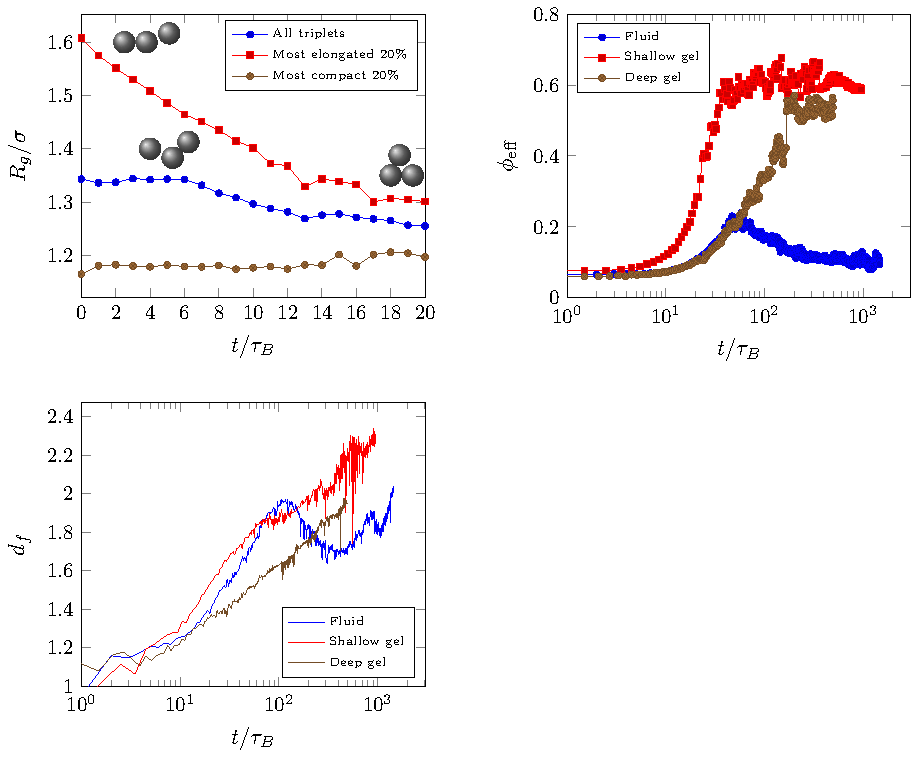
\includegraphics{generate-figure1.pdf}
	\end{center}
	\caption{\textbf{Fluid and dilute gel.} \textbf{a} Compaction mechanism of 3-particle-clusters in a fluid. The characteristic time to reach the stable compact cluster is much longer than $\tau_B$. \textbf{b} Effective volume fraction for various percolating and non-percolating samples. Dilute gels reach effective volume fractions comparable to dense phases due to their lack of compactness. \textbf{c-d} Time-evolution of the fractal dimension of the non-percolation clusters below (\textbf{c}) and above (\textbf{d}) the gelation boundary. Insets: typical $d_f$ plots for various times.}
	\label{fig:fluid_dilute}
\end{figure}

\clearpage
\begin{figure}
	\begin{center}
	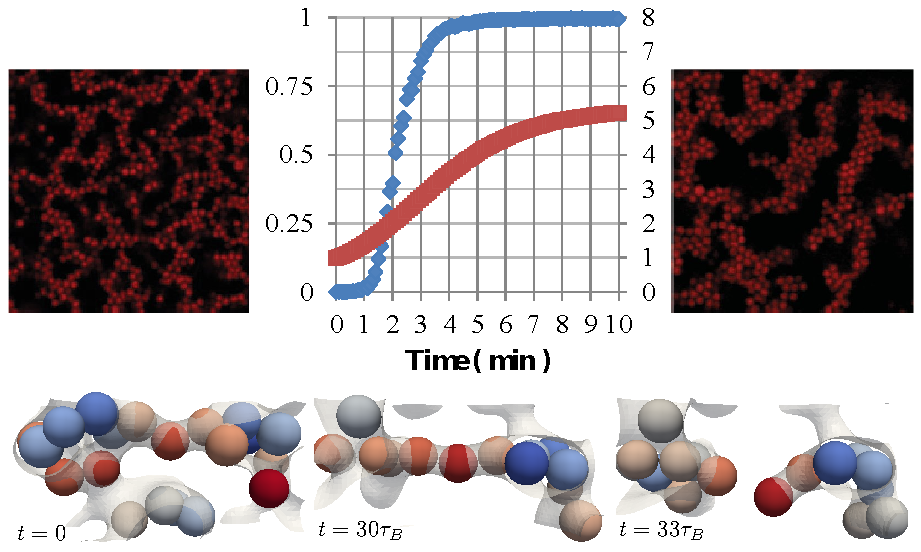
\includegraphics{generate-figure2.pdf}
	\end{center}
	\caption{\textbf{Gelation in dense samples.} \textbf{a} Typical time evolution of the largest cluster size and of the mean coordination number. Insets: Confocal images (2D) at percolation and at final stage. \textbf{b-d} Typical arm-breaking event, from relaxed, to stretched, to rupture. Particles are drawn to scale and colors indicate potential energies from blue (low) to red (high). The smooth surface is a Gaussian coarse-graining of the network pattern. %\textbf{e-f} Typical loop compaction event.  \textbf{b-f} are top views, thus there is no direct role of sedimentation.
	}
	\label{fig:dense}
\end{figure}

\clearpage
\begin{figure}
	\begin{center}
	%\includegraphics{generate-figure3.pdf}
	\end{center}
	\caption{\textbf{Percolation vs compaction} for the three systems studied here: fluid (not percolating), dilute gel and dense gel.}
	\label{fig:general}
\end{figure}
\end{document}